\section{\molmoactt}
\label{sec:molmoact2}

\molmoactt follows a three-stage training pipeline, with the post-training architecture summarized in Fig.~\ref{fig:overview}. Pre-training~(Sec.~\ref{sec:pretraining}) adapts the Molmo2-ER vision-language backbone into a discrete autoregressive robot policy, using the \molmoactfast~(Sec.~\ref{sec:openfast}) to map continuous trajectories into a compact action vocabulary under a unified next-token recipe~(Sec.~\ref{sec:pretraining-recipe}). Post-training~(Sec.~\ref{sec:posttraining}) attaches a flow-matching action expert with per-layer KV conditioning on the autoregressive backbone~(Sec.~\ref{sec:posttraining-action-expert}), and co-trains discrete and continuous action supervision~(Sec.~\ref{sec:posttraining-recipe}) to produce continuous control. Deployment~(Sec.~\ref{sec:deployment}) then covers embodiment-specific fine-tuning~(Sec.~\ref{sec:finetuning}) and inference optimization~(Sec.~\ref{sec:inference}). Shared implementation details for training infrastructure, packing, prompt formatting, and stage-level hyperparameters are provided in \autoref{supp:training}.

\molmoactt is designed around a practical tension: we want to preserve the scaling properties and general visual-language competence of a pretrained VLM, while producing precise continuous robot actions across heterogeneous embodiments. Directly training a VLM and a continuous action expert together from the beginning makes optimization unnecessarily difficult: the model must simultaneously learn a robot-aware token interface, align new state/action embeddings, and fit a flow-matching controller. We therefore use a three-stage pipeline. Pre-training first turns \molmoer into an action-aware VLA using only autoregressive supervision, which gives the backbone aligned robot, state, and action-token embeddings under the same next-token objective used by the base VLM. Post-training then attaches the continuous action expert to this already action-aware backbone, allowing the flow-matching controller and its VLM conditioning interface to align quickly on a broad robot-data mixture. We keep post-training separate from embodiment-specific fine-tuning for efficiency: the post-training mixture is intentionally diverse across datasets, robots, control rates, camera layouts, and task families, so extending it until the model is directly deployment-ready for every target embodiment would require a long and expensive training stage. Instead, post-training produces a general continuous-control base model, and fine-tuning adapts that model quickly to a specific embodiment, environment, and use case while keeping the same architecture and output interfaces.


\subsection{Pre-training}
\label{sec:pretraining}

\molmoacttpre adapts the \molmoer vision-language backbone into a discrete autoregressive robot policy while keeping the Molmo2 token interface intact. Images and video frames are still encoded by a ViT, pooled and projected by the vision-language connector, and passed to the LLM together with text. Robot examples extend this sequence with two additional token streams: state tokens that describe the current robot configuration, and action tokens that describe the future one-second motion.

This subsection focuses on the two ingredients needed to make that formulation practical. First, we describe \molmoactfast, which converts continuous, embodiment-specific robot trajectories into compact discrete action tokens. Second, we describe the pre-training recipe that lets these robot sequences be mixed with standard multimodal data: single-crop visual inputs, a small number of sampled video frames, setup/control and action-output markers, state tokenization, and packed training sequences. Together, these choices preserve a single next-token prediction objective across text, vision-language, state, and action targets, without introducing a separate continuous action head at this stage.

\subsubsection{\molmoactfast}
\label{sec:openfast}

Robot actions are continuous, embodiment-specific, and often produced at different control rates, so they cannot be inserted into a language-model pre-training stream directly. We therefore train \molmoactfast, an open-weight and open-data action tokenizer following FAST~\citep{pertsch2025fast}. The goal is not to introduce a different tokenization principle, but to make this component fully inspectable and reproducible: existing FAST weights are useful, but their training data mixture is not fully specified. \molmoactfast fills this transparency gap by releasing both the tokenizer weights and the action mixture used to train it. It maps a one-second action trajectory into a compact sequence of discrete tokens by representing the trajectory with a frequency-domain transform, quantizing the resulting coefficients, and applying byte-pair encoding to produce tokens from a 2048-token action vocabulary.

Unlike the prior FAST tokenizer, whose released weights are not paired with a fully specified training distribution, \molmoactfast is trained from a transparent action mixture. We subsample one million action sequences across five embodiments, balancing the main \molmoactt deployment platforms with smaller sources that broaden the control vocabulary (\autoref{tab:fast-data}). This gives \molmoactfast coverage over bimanual YAM, SO-100/101, DROID Franka, BC-Z \citep{jang2022bc}, BridgeData V2 \citep{walke2023bridgedata}, RT-1 \citep{brohan2022rt}, and \molmoactdata trajectories, including both absolute joint control and delta end-effector control.

Before fitting the tokenizer, we put all raw robot telemetry into a common action format. Each training sequence corresponds to one second of robot motion, so the number of actions in a chunk is set by the control frequency of the source dataset. Each action in the chunk is padded to 32 dimensions, so embodiments with different action dimensionalities share the same tokenizer input space. Continuous dimensions are normalized with 1--99 percentile statistics, which limits the effect of outliers while preserving the useful dynamic range of each control dimension. Gripper commands are handled separately from this continuous normalization, since they are typically binary or narrow-range open/close signals. This standardized representation allows the same tokenizer to cover both joint-space and end-effector control across multiple robot platforms.

\begin{table}[t]
\centering
\small
\setlength{\tabcolsep}{5pt}
\renewcommand{\arraystretch}{1.05}
\caption{\textbf{Embodiment mixture for \molmoactfast training.} The tokenizer is trained on one million subsampled action sequences spanning the main robot embodiments used by \molmoactt, plus smaller sources that broaden control-mode coverage.}
\label{tab:fast-data}
\begin{tabular}{lcll}
% \toprule
\textbf{Dataset} & \textbf{Mix} & \textbf{Robot} & \textbf{Action representation} \\
\midrule
\molmoacttyamdata & 30\% & YAM & Absolute joint \\
\molmoacttsodata & 30\% & SO-100/101 & Absolute joint \\
\molmoacttdroiddata & 30\% & Franka & Absolute joint \\
Fractal~\citep{brohan2022rt} & 3.33\% & Google Robot & Delta end-effector \\
BC-Z~\citep{jang2022bc} & 3.33\% & Google Robot & Delta end-effector \\
Bridge~\citep{walke2023bridgedata} & 3.33\% & WidowX & Delta end-effector \\
% \bottomrule
\end{tabular}
\end{table}

\subsubsection{Pre-training recipe}
\label{sec:pretraining-recipe}

\paragraph{Model.}
We initialize from the \molmoer checkpoint and keep the Molmo2 vision-language architecture~\citep{clark2026molmo2openweightsdata}. Visual observations are encoded by the SigLIP2 ViT~\citep{tschannen2025siglip}, converted into language-model tokens by the connector, and passed to the LLM together with the language instruction and robot-specific text. The connector uses the same Molmo2 design: features from the third-to-last and ninth-from-last ViT layers are pooled into compact image or video-frame tokens and projected into the LLM embedding space. Full backbone and added-token details are given in \autoref{supp:model-backbone}, with architecture hyperparameters in \autoref{tab:hyperparams_model}.

\paragraph{Data.}
The training mixture combines multimodal examples with robot trajectories so that the model retains vision-language capability while learning to predict actions; we describe the data sources and curation in Sec.~\ref{sec:data}. We allocate 10\% of sampling to multimodal data and 90\% to robot trajectories. Within the robot portion, YAM, SO-100/101, and DROID each receive 30\% of the robot sampling weight; the remaining 10\% is split across smaller BC-Z, BridgeData V2, RT-1, and \molmoactdata sources. For all visual inputs in this stage, we use a single resized crop rather than high-resolution tiled crops. For videos, we sample at most 8 frames at up to 2 FPS, and we skip examples that exceed the sequence budget, which primarily removes unusually long text examples and videos with long captions. We also apply the image augmentation described in \autoref{supp:training} during pre-training, combining light geometric perturbations with color jitter and occasional blur. For multi-camera robot episodes, we randomize the input camera order at the episode level to prevent the model from relying on a fixed camera slot. Each robot example also includes setup and control strings using the same special-token wrappers used during training, e.g., \texttt{\detokenize{<setup_start>bimanual yam robotic arms in molmoact2<setup_end>}}, and \texttt{\detokenize{<control_start>absolute joint pose<control_end>}} or \texttt{\detokenize{<control_start>delta end-effector pose<control_end>}}; the corresponding chat template and output trigger formatting are detailed in \autoref{supp:training}.

\paragraph{Action and state representation.}
This stage is deliberately limited to discrete autoregressive supervision: the model predicts action tokens, but does not yet train the continuous action expert used in post-training. Each robot target is represented as a one-second action chunk, so the number of raw actions in the chunk follows the control frequency of the source dataset. Before tokenization, continuous action and state dimensions are normalized with 1--99 percentile statistics; gripper commands are treated separately from this percentile scaling when they are represented as binary or narrow-range open/close signals. Action vectors are padded to a 32-dimensional space and then encoded with the 2048-token vocabulary of \molmoactfast. Proprioceptive state is represented separately: after normalization, each state value is uniformly discretized into one of 256 state tokens and appended to the prompt before the action target.

\paragraph{Training.}
We train for 200K steps with a maximum sequence length of 4200 tokens. Examples vary substantially in length: a text-only example may use only a few hundred tokens, while multi-camera robot examples must carry images, states, and action targets. We therefore use on-the-fly packing to combine multiple short examples into one 4200-token sequence. Packed examples share the same forward pass, but their text, visual tokens, state tokens, and action targets remain separated by the training attention mask, so the model does not condition one example on another. Appendix~\ref{supp:training} gives the implementation details for this packing procedure and the shared training stack. We train the vision encoder, connector, language model, and newly added tokens' embeddings with a global batch size of 128 across 64 H100 GPUs for around 5,760 GPU hours. The vision encoder and connector use a learning rate of \(5\times10^{-6}\), and the language model uses \(1\times10^{-5}\). This produces a discrete VLA checkpoint that can later be adapted to continuous control.

\subsection{Post-training}
\label{sec:posttraining}



\begin{figure}[t]
\centering
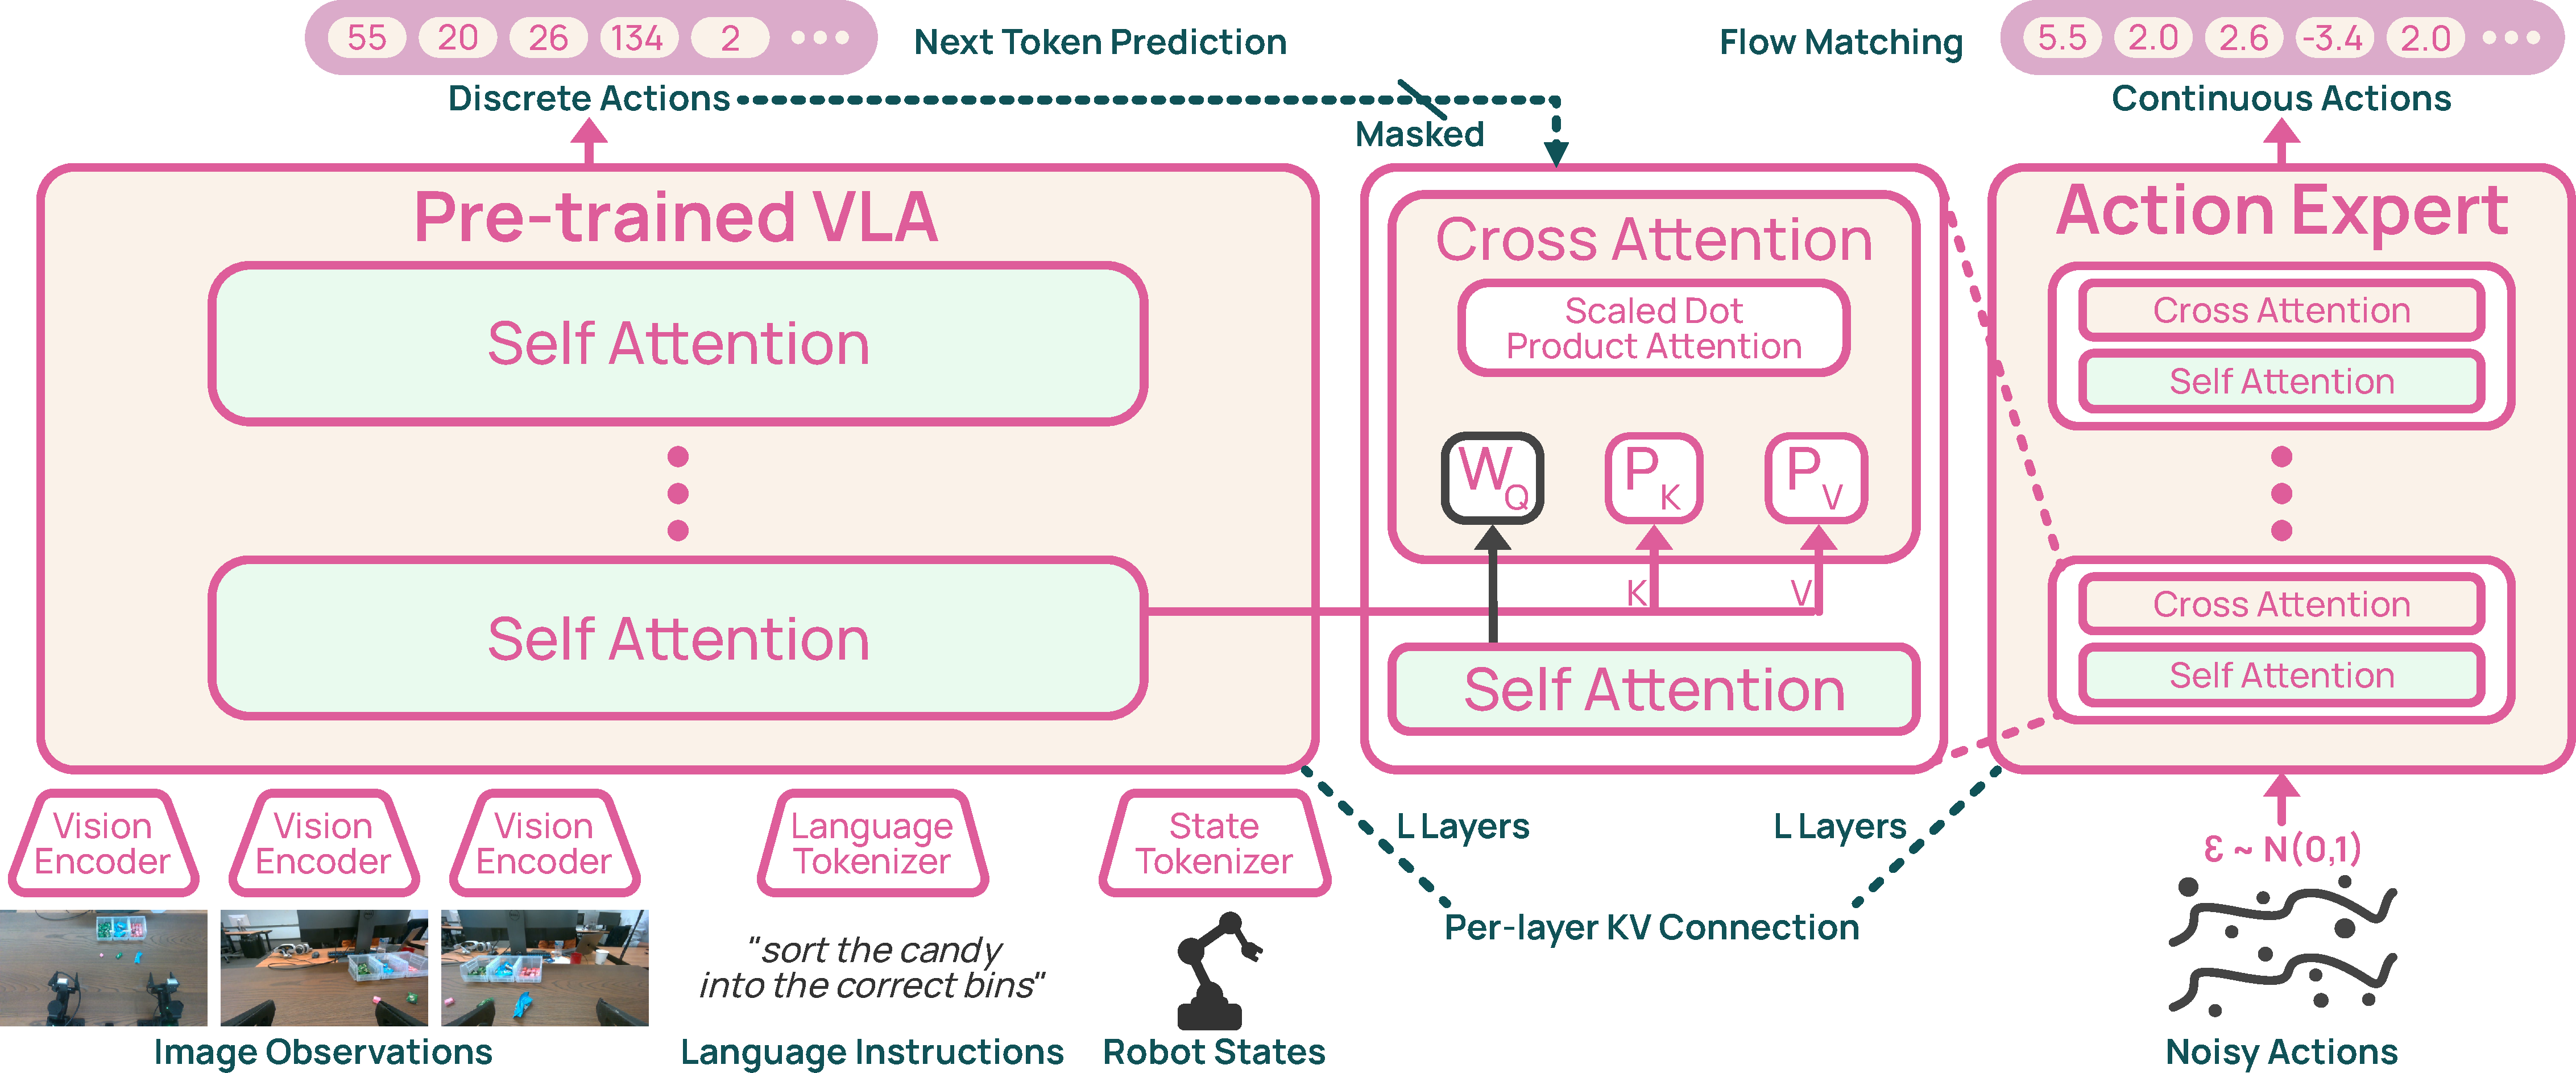
\includegraphics[width=\linewidth]{figures/MAF3.pdf}
\caption{\textbf{Overview of \molmoactt.} Image observations, language
instructions, and robot states are tokenized and processed by a pre-trained
VLA backbone with self-attention layers. Post-training attaches a DiT-style
action expert with the same number of layers as the backbone. At each layer,
the backbone key and value tensors are projected and reused as the key and
value inputs to the action expert's cross-attention, enabling per-layer KV
conditioning from visual-language context to continuous control. The expert is
trained with flow matching to denoise a noisy action trajectory into a
continuous robot trajectory. During training, the backbone is also supervised
with next-token prediction over discrete action tokens, while the target
action-token span is masked from the expert so continuous action prediction
cannot condition on the ground-truth discrete actions.}
\label{fig:overview}
\end{figure}


\molmoacttpre learns a robot policy through the same autoregressive interface used by the VLM: given language, visual observations, setup/control descriptors, and state tokens, it predicts discrete action tokens produced by \molmoactfast. This makes large-scale robot pre-training simple and stable, but the deployed policy should output continuous action trajectories directly. Post-training therefore adds a flow-matching action expert to the pre-trained VLM, producing the final \molmoactt model.

This section describes the two parts of that adaptation. First, we introduce the action expert and its per-layer KV conditioning on the VLM, which lets the continuous controller condition on the full visual-language attention state without replacing the backbone. Second, we describe the post-training recipe: how we keep the pre-training data construction, co-train discrete and continuous action supervision, mask padded or target-leaking tokens, and adjust packing and sequence lengths for the added action-expert compute. Additional model hyperparameters and implementation details are given in \autoref{supp:model-action-expert}, with shared training-system details in \autoref{supp:training}.

\subsubsection{Action expert and per-layer KV conditioning}
\label{sec:posttraining-action-expert}

Post-training adds a continuous action expert on top of the pre-trained autoregressive VLM. We use a DiT-style transformer expert because flow matching and diffusion models have shown that denoising transformers scale well for continuous generation, and because action trajectories are naturally represented as short continuous sequences rather than as text-like token streams. This choice separates responsibilities: the VLM provides visual-language grounding and robot-state context, while the expert models the continuous velocity field needed to transform noisy action chunks into executable trajectories.

The key architectural question is how this expert should receive VLM context. A shallow projection of the final hidden state compresses the backbone into a single residual-stream representation. Instead, \molmoactt conditions the expert on the VLM at every layer. Each action-expert block cross-attends to the corresponding VLM layer's keys and values, after lightweight learned projections map the VLM attention state into the expert's cross-attention width. This gives the continuous controller access to the same attention state used by the VLM itself, while preserving a modular interface between the backbone computation and the newly trained action expert.

Given a normalized target action chunk \(a\), Gaussian noise \(\epsilon\), and a sampled time \(t \in [0,1]\), we interpolate between noise and data,
\begin{equation}
    x_t = (1-t)\epsilon + t a,
    \qquad
    u^\star = a - \epsilon.
\end{equation}
The expert \(f_\theta\) predicts the target velocity \(u^\star\) from the noisy action chunk, the time embedding, and the VLM context \(c\), which contains the task, visual observations, setup/control descriptors, and discrete state tokens:
\begin{equation}
    \mathcal{L}_{\mathrm{flow}}
    =
    \mathbb{E}_{a,\epsilon,t}
    \left[
    \left\|
    m \odot \left(f_\theta(x_t,t,c) - u^\star\right)
    \right\|_2^2
    \right],
\end{equation}
where \(m\) masks padded action steps and padded action dimensions. At inference, we start from Gaussian noise and integrate the predicted velocity field to produce a continuous action trajectory.

Architecturally, the expert has the same depth as the VLM, where both of them use \(L=36\) layers. The expert first embeds the current noisy action sequence. Each block then applies action self-attention, cross-attention to the VLM, and an MLP, with the time embedding producing DiT-style shift, scale, and gate parameters for all three residual branches. Schematically, block \(\ell\) computes
\begin{align}
    h'_\ell
        &= h_\ell + g^{\mathrm{sa}}_\ell
        \operatorname{SA}\!\left(\operatorname{AdaRMS}^{\mathrm{sa}}_\ell(h_\ell,t)\right), \\
    \bar{h}_\ell
        &= h'_\ell + g^{\mathrm{ca}}_\ell
        \operatorname{CA}\!\left(
            \operatorname{AdaRMS}^{\mathrm{ca}}_\ell(h'_\ell,t),
            \tilde{K}_\ell,
            \tilde{V}_\ell
        \right), \\
    h_{\ell+1}
        &= \bar{h}_\ell + g^{\mathrm{ff}}_\ell
        \operatorname{MLP}\!\left(\operatorname{AdaRMS}^{\mathrm{ff}}_\ell(\bar{h}_\ell,t)\right).
\end{align}

The action expert uses per-layer KV conditioning rather than hidden-state conditioning. For each VLM layer \(\ell\), we collect the keys and values \((K^{\mathrm{vlm}}_\ell,V^{\mathrm{vlm}}_\ell)\) produced by that layer's self-attention. We then project them into the action-expert width with learned adapter projections \(P_K\) and \(P_V\):
\begin{equation}
    \tilde{K}_\ell =
    \operatorname{reshape}\!\left(P_K K^{\mathrm{vlm}}_\ell\right),
    \qquad
    \tilde{V}_\ell =
    \operatorname{reshape}\!\left(P_V V^{\mathrm{vlm}}_\ell\right).
\end{equation}
Here, \(P_K\) and \(P_V\) are linear VLM-to-expert adapter layers that align the VLM KV dimensionality with the expert's cross-attention width; they are separate from the VLM self-attention projections that produced the keys and values. After projection, the conditioning context is organized into the expert's attention heads. The cross-attention in expert block \(\ell\) attends to the projected keys and values from the corresponding VLM layer:
\begin{equation}
    \operatorname{CA}(Q_\ell,\tilde{K}_\ell,\tilde{V}_\ell)
    =
    \operatorname{softmax}\!\left(
        \frac{Q_\ell \tilde{K}_\ell^\top}{\sqrt{d_h}}
    \right)\tilde{V}_\ell,
\end{equation}
where \(d_h\) is the expert head dimension. This per-layer KV conditioning gives every action-expert block direct access to the visual-language attention state at the same depth in the backbone. During post-training we detach this conditioning path from the VLM, so the flow loss trains the expert and its adapter projections without sending gradients back through the VLM keys and values.

\subsubsection{Post-training recipe}
\label{sec:posttraining-recipe}

\paragraph{Overview.}
Post-training starts from the 200K-step \molmoacttpre checkpoint and turns it into the final \molmoactt model. We keep the VLM architecture and pre-training data construction from Sec.~\ref{sec:pretraining-recipe}, including the image augmentation described in \autoref{supp:training}. The main change is that robot examples now supervise both output interfaces: the LLM continues to predict discrete action tokens, while the action expert described in Sec.~\ref{sec:posttraining-action-expert} learns to generate continuous action chunks.

\paragraph{Multiple flow samples.}
For each robot action chunk, we evaluate the flow objective at multiple noise levels. Let \(a\) be a normalized continuous action chunk and \(c\) be the VLM context for the corresponding robot prompt. For each training example we draw \(K\) independent pairs \(\{(\epsilon_i,t_i)\}_{i=1}^K\), form \(x_{t_i}=(1-t_i)\epsilon_i+t_i a\), and train the expert to predict \(a-\epsilon_i\):
\begin{equation}
    \mathcal{L}_{\mathrm{flow}}(a,c)
    =
    \frac{1}{K}
    \sum_{i=1}^{K}
    \left\|
    m \odot
    \left(
    f_\theta(x_{t_i},t_i,c) - (a-\epsilon_i)
    \right)
    \right\|_2^2 .
\end{equation}
We use \(K=4\), so each robot sample contributes four points on the same flow trajectory while reusing the same visual-language context. We didn't use \(K=8\) as in the fine-tuning stage (Sec.~\ref{sec:finetuning}) mainly due to GPU memory constraints.

\paragraph{Padding and packing.}
Post-training retains a common action tensor shape across embodiments. Continuous actions are right-padded to a maximum horizon of 30 steps and a maximum width of 32 dimensions. The horizon mask removes padded time steps from the flow loss, and the dimension mask zeroes padded action dimensions in the noisy inputs, targets, and predictions before averaging the loss over valid dimensions. This lets datasets with different control rates and action widths share the same expert without training on artificial padded coordinates.

Packing is also extended to the continuous expert. A packed language sequence can contain multiple robot examples; each action chunk is paired with the sub-example that produced it, and the expert attends only to that example's VLM context. To keep memory use stable when packed batches contain different numbers of robot chunks, we pad the packed action-chunk axis up to a small fixed cap of five chunks per packed sequence when possible. Padded chunk rows are marked invalid and excluded from the flow loss; sequences with more chunks are still used, but processed without this fixed-cap padding.

\paragraph{Training objectives.}
The post-training objective combines the autoregressive loss from pre-training with the flow-matching loss:
\begin{equation}
    \mathcal{L}_{\mathrm{post}}
    =
    \mathcal{L}_{\mathrm{LM}}
    +
    \mathcal{L}_{\mathrm{flow}} .
\end{equation}
The language-model loss is applied to the same next-token targets used in pre-training, including discrete action tokens for robot examples and text tokens for VLM examples. The flow loss is applied only to continuous robot action chunks. Since robot examples contain both the discrete action target and the continuous action target, we mask the discrete action-token span out of the expert's VLM conditioning path. The expert therefore conditions on the task, observations, setup/control descriptors, and state tokens, but not on the target action tokens it is supposed to predict.

We also apply knowledge insulation \citep{driess2025knowledgeinsulation}, where the VLM is isolated from the continuous-action loss. The expert conditions on the VLM keys and values, but these tensors are detached before they enter the expert, so \(\mathcal{L}_{\mathrm{flow}}\) updates the action expert and its adapter projections without back-propagating through the VLM. The VLM is still updated by \(\mathcal{L}_{\mathrm{LM}}\).

\paragraph{Training.}
Robot batches use a sequence length of 2100 tokens, while the non-robot VLM batches keep the 4200-token context length from pre-training. We use this split because robot batches additionally run the action expert and four flow samples per action chunk, whereas VLM batches only train the autoregressive model. We train for 100K updates with a global batch size of 128 and a device batch size of 2 across 64 H100 GPUs for around 2,304 GPU hours. The VLM learning rates match pre-training: \(5\times10^{-6}\) for the vision encoder and connector, and \(1\times10^{-5}\) for the language model. The action expert is trained with a larger learning rate of \(5\times10^{-5}\).


\subsection{Deployment}
\label{sec:deployment}

\subsubsection{Embodiment-specific fine-tuning}
\label{sec:finetuning}



\paragraph{Shared recipe.}
Embodiment-specific fine-tuning starts from the post-trained \molmoacttpos checkpoint and keeps the same VLM--action-expert architecture described in Sec.~\ref{sec:posttraining}. We continue to co-train the discrete autoregressive action output and the continuous flow-matching action expert, use the same 32-dimensional padded action width, and keep the same learning rates as post-training: \(5\times10^{-6}\) for the vision encoder and connector, \(1\times10^{-5}\) for the language model, and \(5\times10^{-5}\) for the action expert. We also keep single resized crops, packed sequences, setup/control descriptors, discrete state tokens, and the same action-token vocabulary, using the shared prompt, image-augmentation, and packing implementation described in \autoref{supp:training}.

The fine-tuning stage differs from post-training in four ways. First, each run is robot-only: we do not include the multimodal VLM mixture or a separate VLM dataloader. Second, we increase the number of sampled flow times from 4 to 8 per action chunk, which gives the action expert denser supervision along the same flow trajectory. Third, we do not use knowledge insulation during fine-tuning: gradients from the flow loss are allowed to update the VLM through the action-expert conditioning path, since we did not observe a consistent performance gain from detaching this path at this stage. Finally, for the main embodiment checkpoints below, we do not tune the added-token input embeddings. As in standard VLM fine-tuning, we assume that the token embeddings learned during pre-training and post-training are already well placed, and tune the language-model output head and final normalization instead.

\paragraph{Bimanual YAM.}
The \molmoacttyam checkpoint is fine-tuned on the bimanual YAM mixture. The camera order is fixed as top, left, and right, matching the data collection setup. We use annotated language instructions, absolute joint-pose actions, and a 30-step action chunk, corresponding to the 30 Hz control rate of the dataset. We train with a sequence length of 2100, global batch size 128, and 100K updates on 64 H100 GPUs, for roughly 2,304 GPU hours.

\paragraph{DROID.}
The \molmoacttdroid checkpoint is fine-tuned on the filtered DROID mixture. DROID provides two exterior cameras and one wrist camera. For DROID-style two-view evaluation, we use a fixed exterior-then-wrist ordering; when training variants expose both exterior choices as alternatives, the loader samples one exterior camera and pairs it with the wrist camera during training. We use absolute joint-pose actions with a 15-step action chunk, matching DROID's 15 Hz control rate. We do not use the additional language annotations in this fine-tune, to keep the comparison with prior DROID-trained models fair. We train with a sequence length of 2100, global batch size 64, and 100K updates on 32 H100 GPUs, for roughly 1,152 GPU hours.

\paragraph{SO-100/101.}
The \molmoacttso checkpoint is fine-tuned on the SO-100/101 mixture. Because this data is aggregated from internet demonstrations with diverse and inconsistent camera layouts, we randomize the input camera order at the episode level rather than imposing a fixed view naming convention. We use annotated language instructions, absolute joint-pose actions, and a 30-step action chunk for the 30 Hz control rate. We train with a sequence length of 2100, global batch size 64, and 100K updates on 32 H100 GPUs, for roughly 1,152 GPU hours.

\paragraph{LIBERO.}
The \molmoacttlib checkpoint is fine-tuned on the full LIBERO training mixture, combining the Spatial, Object, Goal, and Long suites rather than training a separate model for each suite. The camera order is fixed as front view followed by wrist view. We do not use annotated language instructions. LIBERO uses relative end-effector control at 10 Hz, so we train with a 10-step action chunk. We use a sequence length of 2100, global batch size 64, and train for 50K updates on 32 H100 GPUs, for roughly 1,152 GPU hours; for evaluation, we select the best-performing checkpoint, which occurs at 40K updates.

\paragraph{Other evaluation fine-tunes.}
For smaller task- or benchmark-specific fine-tunes used in downstream evaluation, we follow the same recipe unless otherwise noted. These runs use fixed metadata camera order rather than camera-order randomization, no language annotations, 2100-token sequences, packing, 8 sampled flow times, and robot-only data. The action horizon is set to the dataset control frequency, and the control representation follows the dataset, either joint pose or end-effector pose. Real-world evaluation runs use 8 H100 GPUs, global batch size 16, and 50K updates, and we choose the best-performing checkpoint for evaluation.

\subsubsection{Inference optimization}
\label{sec:inference}
For the \molmoactt model, inference is dominated by the continuous action expert, which integrates a fixed-step flow-matching trajectory conditioned on the VLM context. Within one action chunk, this context is invariant across flow steps, while only the noisy action state and flow time evolve. We therefore cache reusable action-expert intermediates, including context-dependent cross-attention states and fixed position-dependent terms, and reuse them throughout the flow loop. We further capture the fixed-shape flow loop with CUDA Graphs, reducing Python and kernel-launch overhead during repeated action generation.

